\subsubsection{Distributing the discs randomly in $[0,1]\times[0,0.5]$}

To distribute the particles randomly in the box defined by 
$$
\{(x,y)\in \RR : 0 < x < 1, 0 < y < 0.5\}
$$ 
I use the following scheme. 

To choose a suitable radius to have the particles fill up the available space with a packing fraction of $\rho \approx 1/2$ I solve for $r$ in 
$$
	N \pi r^2 = A(r) \rho = \frac{1}{2} A(r),  
$$
where, in order to avoid having particles outside the box, the area depends on $r$. If we clear a border of $r$ on the boundary of the region facing the walls, we get $r$ from solving

\begin{equation}\label{eq:r}
	N \pi r^2 = \frac{1}{2} (1- \frac{1}{2}2) (1-2r \quad \Rightarrow \quad r = \frac{-1 + \sqrt{N\pi}}{2(N\pi - 1)}.
\end{equation}

To avoid having overlapping particles, I do the following

\begin{algorithm}[H]
	Choose number of particles $N$\;
	Find $r$ corresponding to $N$ from \eqref{eq:r}\;
	$\mathbf{x} \gets [(0,0),\dots,(0,0)]$\;
	$\mathbf{x}_0 \gets (x_i \sim \mathcal{U}_{[r,1-r]},y_i \sim \mathcal{U}_{[r,0.5]})$\;
	\For{$i = 2\dots N$ }{
		$\mathbf{x}_i \gets (x_i \sim \mathcal{U}_{[r,1-r]},y_i \sim \mathcal{U}_{[r,0.5]})$\;
	\While{Particle $i$ does not overlap with particle $1,\dots,i-1$}{
		$\mathbf{x}_i \gets (x_i \sim \mathcal{U}_{[r,1-r]},y_i \sim \mathcal{U}_{[r,0.5]})$\;
	}}
	\caption{Event driven simulation of a gas.}
\end{algorithm}  


\subsubsection{Scanning over the projectile mass}

By simulating crater formation with projectile masses running from $1$ to $25$ times the mass of the remaining particles, the size of the crater is as shown in figure \ref{fig:mass_size}. The size of the crater $\mathcal{S}$ is simply the number of particles involved in the crater formation. The plot clearly shows that a larger projectile mass gives rise to a larger crater, as one intuitively would expect. 

\begin{figure}
	\centering
	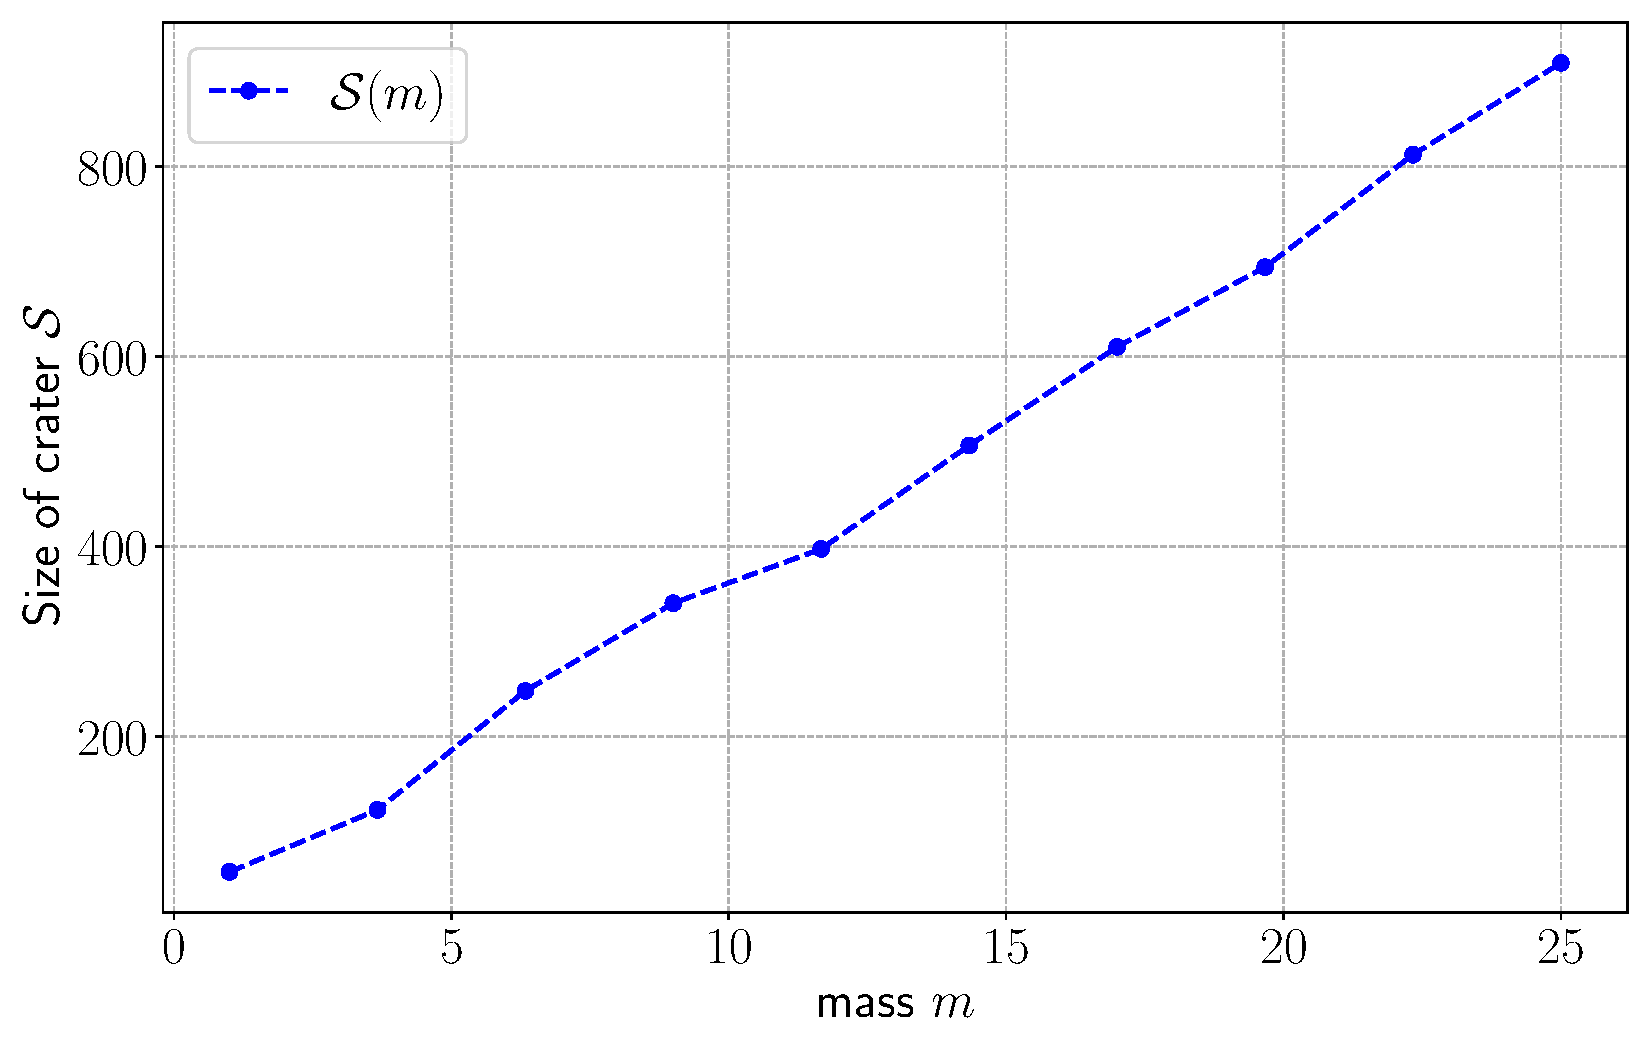
\includegraphics[width=\columnwidth]{../fig/mass_size}
	\caption{Size of crater as a function of projectile mass.}
	\label{fig:mass_size}
\end{figure}